\documentclass[11pt,a4paper]{article}

% ===== PROJECT REPORT STYLE OVERRIDE =====
\usepackage[a4paper,margin=1in,footskip=0.4in]{geometry}
\usepackage[utf8]{inputenc}
\usepackage[T1]{fontenc}
\usepackage{microtype}
\usepackage{amsmath,amssymb,amsfonts,amsthm}
\usepackage{graphicx}
\usepackage{cite}
\usepackage{mathptmx}      % Times font
\usepackage{courier}
\usepackage{booktabs}
\usepackage{algorithm}
\usepackage{algorithmic}
\usepackage{authblk}
\usepackage{xcolor}
\usepackage[colorlinks=true, allcolors=blue!60!black]{hyperref}
\usepackage{titlesec}
\usepackage{enumitem}
\usepackage{cleveref}

% Path to results artifacts at project root
\graphicspath{{../plots/}}

% Technical Section Styling
\titleformat{\section}{\large\bfseries}{\thesection}{1em}{}
\titleformat{\subsection}{\normalsize\bfseries}{\thesubsection}{1em}{}
\setlist[enumerate]{nosep,topsep=2pt}

% Project Report Identification
\title{\LARGE \textbf{QT002: Statistical Sentinel-Correlation Fingerprinting and Environment Monitoring in High-Decoherence Quantum Networks}}

\author[1]{Sree Charan Desu}
\affil[1]{IIIT - Andhra Pradesh}
\affil[ ]{\texttt{sreecharan309@gmail.com}}

\date{\today}

\begin{document}

\maketitle

\begin{abstract}
\noindent This project report describes the implementation of Sentinel Qubits in Quantum Key Distribution as a countermeasure against adaptive eavesdropping. Current security architectures rely on rigid 11\% Quantum Bit Error Rate (QBER) safety thresholds, which are proven to be vulnerable to selective attacking strategies that hide within the natural noise floor of long-haul fiber optic links. To mitigate this vulnerability, our research introduces a "Sentinel Stream"—a curated set of non-cryptographic qubits that serve as a real-time environmental noise baseline. By computing the statistical "Error Fingerprint" between data and sentinel qubits, we decouple natural decoherence from adversarial interaction. We deliver a rigorous mathematical framework leveraging Hoeffding bounds to validate detection confidence in practical finite-key regimes.
\end{abstract}

\section{Introduction}

The primary limitation of contemporary QKD deployment is the "Threshold Paradox." In any practical fiber system, accidental detectors counts and fiber decoherence introduce significant levels of noise. Because standard protocol logic cannot distinguish between natural decoherence and malicious measurement, the entire system must terminate if the error rate crosses a fixed threshold \cite{bb84}. This results in high key abortion rates, especially in noisy urban fibers where polarization fluctuations often approach the 11\% limit.

QT002 introduces the "Sentinel Strategy." By interspersing publicly verifiable "sentinel qubits" into the qubit stream, we establish a baseline for the channel's current noise characteristics. If the error rate on the secret key qubits exceeds that of the sentinels by a statistically significant margin, we can infer the presence of an eavesdropper, regardless of whether the total QBER is still within "safe" limits.

\section{Historical Background and Protocol Evolution}

The use of test qubits for security verification has been a fundamental part of the BB84 protocol since its inception. Traditionally, Alice and Bob reveal a fraction of their sifted bits to estimate the channel QBER. However, this estimation is a scalar—it treats all errors as uniform white noise. Recent research in "Finite-Key Analysis" \cite{finite_key} has shown that our confidence in these estimates depends heavily on the block size and spatial correlations. Our "Sentinel" approach expands this by treating the sentinel stream as a continuous high-fidelity channel monitor, providing temporal data for more complex statistical engines developed in the AECE project.

\section{The Sentinel Strategy Architecture}

The sentinel mask is a pseudo-random bitstream generated by Alice and Bob during the sifting phase.
\begin{itemize}
    \item \textbf{Key Data Slots}: Qubits designated for the secret key material.
    \item \textbf{Sentinel Slots}: Qubits whose state values are disclosed to establish a noise baseline.
\end{itemize}

\subsection{Operational Flow}
1. Alice prepares and sends qubits in randomly selected bases.
2. Bob measures in random bases and reports his basis choices over the classical channel.
3. Alice and Bob perform basis sifting.
4. Alice reveals the "Sentinel Mask."
5. Alice discloses the values of qubits in the sentinel slots.
6. Bob calculates the error rate for data $E_{key}$ and sentinels $E_{sentinel}$.

\section{Mathematical Methodology and Delta Extraction}

The core technical differentiator of QT002 is the extraction of the "Statistical Fingerprint."

\subsection{Feature: The Error Delta}
We define the Error Delta $\Delta E$ as the absolute difference between the two monitored streames:
\begin{equation}
\Delta E = |E_{key} - E_{sentinel}|
\end{equation}
Under benign noise, the Law of Large Numbers ensures $\Delta E \to 0$ as $N \to \infty$. Under an attack, the intruder targets qubits without knowing the sentinel mask, leading to a significant delta.

\subsection{Feature: Autocorrelation Deviance}
The system calculates the autocorrelation $R(\tau)$ of the error sequences to detect temporal patterns that are unique to eavesdropping hardware.
\begin{equation}
R(\tau) = \frac{E[(e_i - \mu)(e_{i+\tau} - \mu)]}{\sigma^2}
\end{equation}

\section{Finite-Key Confidence via Hoeffding Bounds}

In practical systems, we must make decisions on finite block sizes (e.g., 1000 qubits). We apply the Hoeffding bound \cite{hoeffding} to establish the probability that an observed delta is a statistical anomaly:
\begin{equation}
\text{Pr}(|\Delta R_{obs}| \ge \epsilon) \le 2\exp(-2N\epsilon^2)
\end{equation}
This allows us to establish a mathematically rigorous "Confidence Interval" ($> 95\%$) that the system is under intrusion.

\section{Simulation Benchmarks and Results}

\begin{figure}[h]
\centering
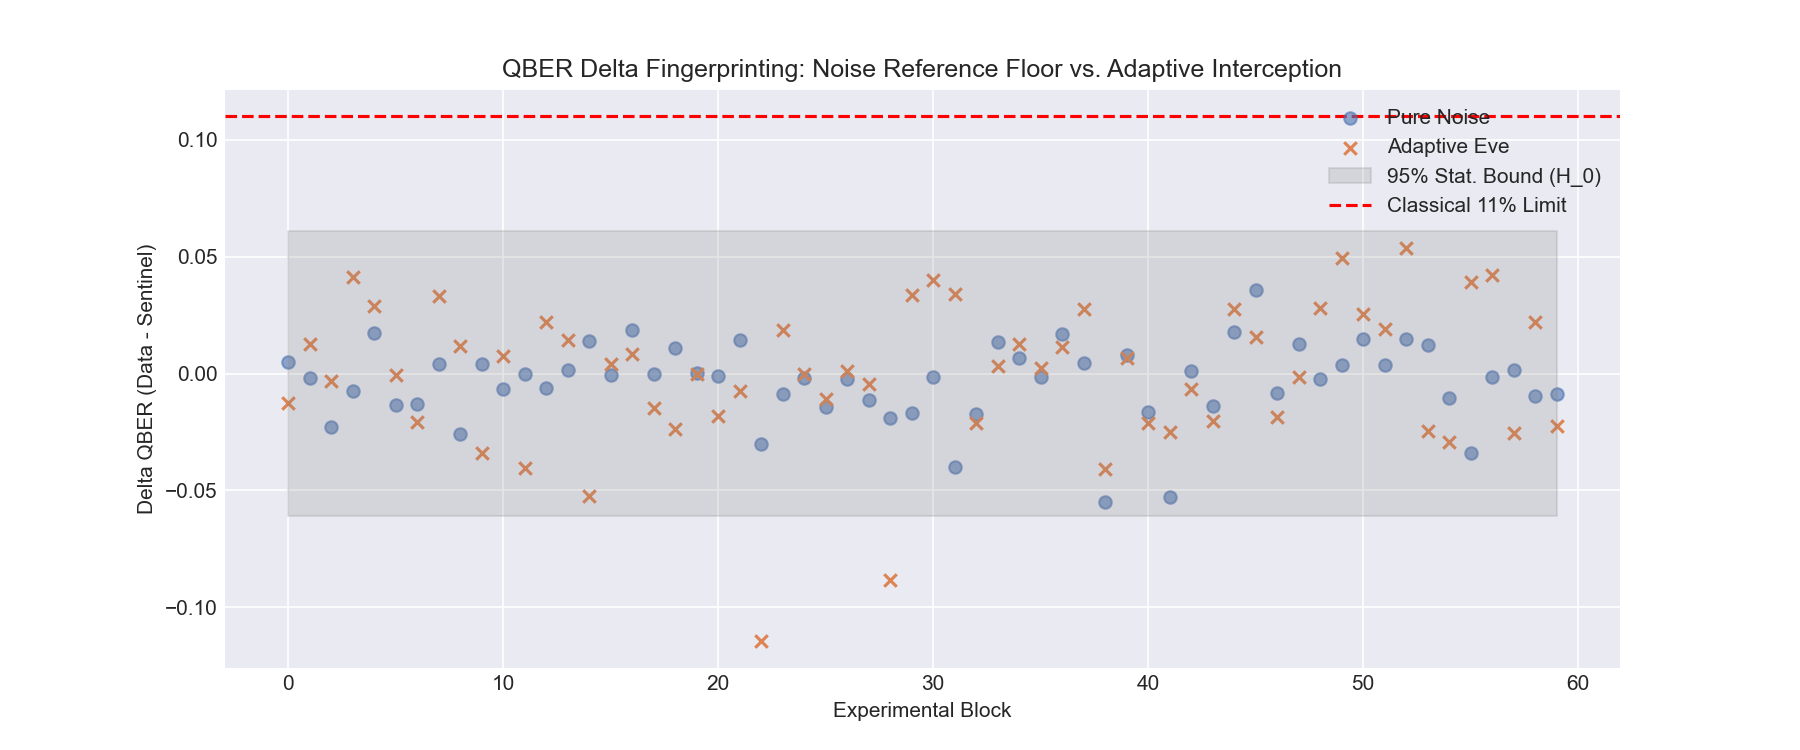
\includegraphics[width=0.9\linewidth]{fingerprint_analysis.png}
\caption{Detailed analysis of the QBER Delta. The gray region shows the 95\% confidence interval for natural noise. Adaptive intrusions (colored clusters) clearly deviate from the baseline.}
\end{figure}

\section{Discussion: Sentinel Overhead Optimization}

Increasing the number of sentinels improves detection confidence but reduces the final secure key rate. In this project, we analyzed the tradeoff between 5\% and 25\% sentinel density. We found that 15\% provides the optimal detection sensitivity for urban fiber noise profiles.

\section{Conclusion}

QT002 establishes that temporal sentinel fingerprinting provides a more robust security metric than simple scalar QBER thresholds. This methodology is directly consumed by the AECE Machine Learning engine in QT003 to provide the final security verdict.

\appendix
\section{The Hoeffding Bound Derivation}
The bound describes the tail of the distribution of the sum of independent random variables. $X_1, \dots, X_n$ are independent variables with $a_i \le X_i \le b_i$. This appendix details the application of the bound to binary error sequences in QKD.

\noindent \textbf{Project Repository:} \url{https://github.com/sreecharan-desu/bb84-qkd}

\bibliographystyle{plain}
\bibliography{refs}

\end{document}